\section{Технический проект}

\subsection{Архитектура программной системы}
Программная система «Цифровая платформа Курский край» реализована по архитектуре «клиент--сервер».
Клиентская часть представлена веб-интерфейсом на HTML/CSS/JavaScript,
который открывается в браузере пользователя. Серверная часть реализована на
Node.js (Express) и предоставляет REST API для чтения и изменения данных.
Хранение данных выполняется в СУБД PostgreSQL.

Выбор такой архитектуры обоснован требованиями проекта: необходимо обеспечить
одновременную работу пользовательской части (просмотр мест, маршрутов, фото)
и административной части (управление объектами и маршрутами) с единой базой
данных. Сервер централизует бизнес-логику, валидацию, а также контроль
доступности опубликованного контента.

Общая схема взаимодействия компонентов приведена на рисунке~\ref{fig:arch-overall}.

\begin{figure}[H]
	\centering
	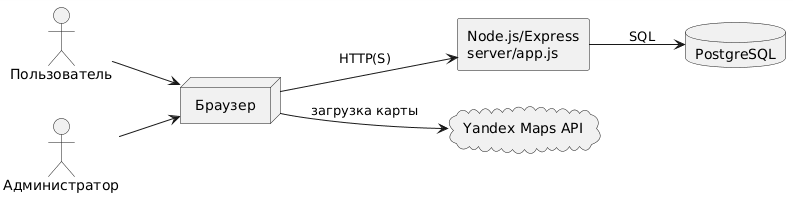
\includegraphics[width=0.85\linewidth, height=4.5cm]{images/arch-overall}
	\caption{Общая схема взаимодействия компонентов}
	\label{fig:arch-overall}
\end{figure}

Серверное приложение обрабатывает HTTP-запросы, маршрутизирует их по эндпоинтам
\texttt{/api/categories}, \texttt{/api/places}, \texttt{/api/routes}, выполняет SQL-запросы к PostgreSQL и
возвращает клиенту данные в формате JSON. Статические страницы пользовательского
и административного интерфейса раздаются тем же Node.js-приложением.

\subsection{Обоснование выбора технологий проектирования}
При выборе технологического стека учитывались требования простоты запуска,
поддерживаемости, возможности работы с картографическими данными и
транзакционного хранения сведений о местах и маршрутах. Выбранный стек
состоит из Node.js/Express на сервере, чистого JavaScript на клиенте,
PostgreSQL в качестве СУБД и Yandex Maps API для отображения карт.

\subsubsection{JavaScript (Node.js) как серверная платформа}
Использование Node.js обосновано тем, что проект использует единый язык
(JavaScript) на клиенте и сервере, что упрощает сопровождение и снижает
порог входа при доработках. Асинхронная модель Node.js подходит для
обработки множества параллельных HTTP-запросов.

Node.js/Express обеспечивает быстрый старт разработки, прозрачную маршрутизацию
и единый язык на фронтенде и бэкенде. Это сокращает стоимость сопровождения и
ускоряет внедрение изменений.

При этом у выбранного стека есть инженерные ограничения:
\begin{enumerate}
	\item Однопоточная event-loop модель чувствительна к блокирующим CPU-операциям.
	\item Типизация JavaScript по умолчанию слабее строготипизированных языков.
	\item Рост проекта требует дополнительной дисциплины архитектурных границ
	(слои, контракты, тесты), иначе возрастает риск «разрастания» контроллеров.
\end{enumerate}

В рамках текущего проекта эти недостатки компенсируются:
\begin{itemize}
	\item выносом тяжёлой логики в SQL и транзакции БД;
	\item модульной структурой клиентского и серверного кода;
	\item строгими API-контрактами и единообразной обработкой ошибок.
\end{itemize}

\subsubsection{Express как веб-фреймворк}
Express выбран как минималистичный и расширяемый фреймворк,
предоставляющий:
\begin{itemize}
	\item маршрутизацию HTTP-запросов;
	\item middleware-подход для обработки JSON и ошибок;
	\item удобную интеграцию с раздачей статических файлов.
\end{itemize}

\subsubsection{PostgreSQL как СУБД}
PostgreSQL обеспечивает транзакционность, ограничения целостности,
надёжную работу с внешними ключами и удобные средства агрегации данных,
которые используются при формировании структур маршрутов с точками.

PostgreSQL выбран как промышленная СУБД с развитой поддержкой транзакций,
ограничений целостности и JSON-операций. Для проекта, где одновременно используются
структурированные сущности (места/маршруты) и вложенные коллекции (галерея,
агрегированные точки маршрута), такой баланс особенно важен.

Альтернативы и их ограничения для данного контекста:
\begin{enumerate}
	\item SQLite: простота развёртывания, но ограниченная модель конкурентной записи
	при интенсивной административной работе.
	\item MySQL/MariaDB: сопоставимая функциональность, но потребовалась бы отдельная
	адаптация SQL-диалекта и миграций под уже выбранный стек.
	\item NoSQL-подход: удобен для документов, но усложняет строгую целостность
	связей маршрутов и мест при требованиях предсказуемой реляционной модели.
\end{enumerate}

Следовательно, PostgreSQL является технически обоснованным компромиссом между
надёжностью, выразительностью запросов и устойчивостью к росту проекта.

\subsubsection{Vanilla JavaScript на клиенте}
Клиентская часть реализована без тяжёлых frontend-фреймворков.
Это снижает сложность сборки, упрощает развёртывание и хорошо подходит
для проекта с акцентом на справочный интерфейс и CRUD-операции.

Отказ от крупного frontend-фреймворка снижает порог сопровождения и убирает
сложность build-пайплайна. Для проекта с умеренной интерактивностью это
рационально: критическая ценность лежит в контенте и карте, а не в сложной
реактивной UI-модели.

Ограничения такого выбора:
\begin{itemize}
	\item при масштабировании интерфейса возрастает объём ручного управления состоянием;
	\item выше риск дублирования DOM-логики между страницами;
	\item сложнее унифицировать паттерны жизненного цикла компонентов.
\end{itemize}

В техническом проекте эти риски адресуются через модульную декомпозицию
(страничные модули и общий слой \texttt{places-store.js} и API-обёртки).

\subsubsection{Интеграция с Yandex Maps API}
Для картографической функциональности использован Yandex Maps API,
что позволяет:
\begin{itemize}
	\item отображать объекты на карте;
	\item выбирать координаты в административном интерфейсе;
	\item визуализировать маршруты в пользовательской части.
\end{itemize}

Использование готового картографического API уменьшает объём собственной
разработки и позволяет сосредоточиться на предметной логике проекта: хранении
объектов, управлении маршрутами и отображении туристического контента.

\subsection{Клиентская часть}
Структура клиентского слоя включает HTML-страницы и
набор JS-модулей, каждый из которых отвечает за свой сценарий работы.

Назначение HTML-страниц определяется следующим образом:
\begin{enumerate}
	\item Страница \texttt{index.html} является входной точкой пользовательского интерфейса и содержит обзорный экран проекта.
	\item Страница \texttt{places.html} предназначена для просмотра каталога мест, фильтрации по категориям и открытия карточек объектов.
	\item Страница \texttt{routes.html} используется для отображения маршрутов, состава точек маршрута и связанных объектов.
	\item Страница \texttt{photos.html} реализует фотогалерею и переходы к карточкам мест по выбранным изображениям.
	\item Страница \texttt{admin.html} предназначена для административных операций: создания, редактирования и удаления категорий, объектов и маршрутов.
\end{enumerate}

Назначение основных JavaScript-файлов следующее:
\begin{enumerate}
	\item Модуль \texttt{places-page.js} загружает данные каталога мест через API, применяет фильтры и управляет визуализацией карточек.
	\item Модуль \texttt{routes-page.js} запрашивает маршруты, строит структуру точек и отображает связанный маршрутный контент.
	\item Модуль \texttt{photos-page.js} подготавливает данные галереи и обрабатывает переходы пользователя между фото и карточками объектов.
	\item Модуль \texttt{admin-page.js} реализует формы CRUD-операций, валидацию перед отправкой и синхронизацию таблиц после изменений.
	\item Модуль \texttt{api\_places.js} инкапсулирует HTTP-вызовы к серверным endpoint-ам и унифицирует обработку ответов.
	\item Модуль \texttt{places-store.js} хранит клиентское состояние каталога и промежуточные структуры для фильтрации.
	\item Модуль \texttt{theme.js} отвечает за переключение темы и сохранение пользовательских настроек отображения.
\end{enumerate}

Диаграмма компонентов клиентской части приведена на рисунке~\ref{fig:arch-client}.

\begin{figure}[H]
	\centering
	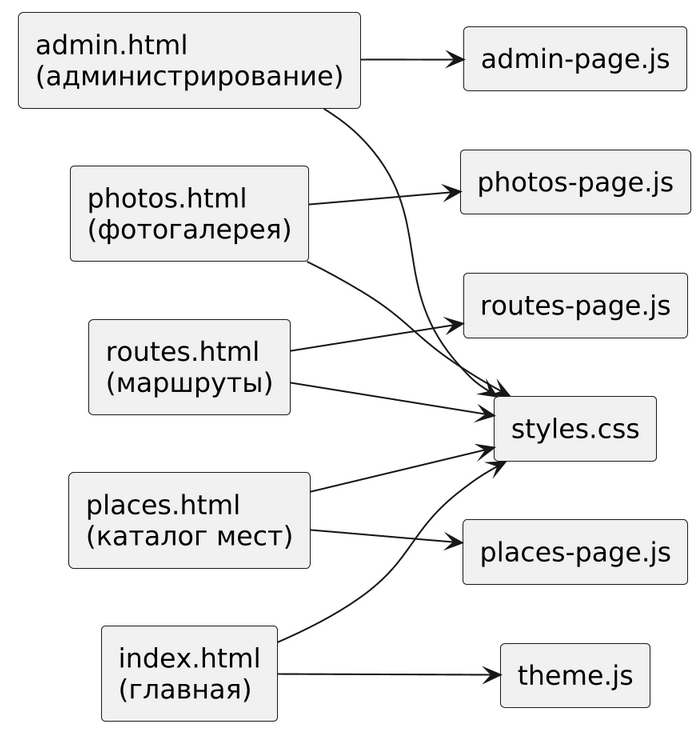
\includegraphics[width=0.5\linewidth, height=10cm]{images/arch-client}
	\caption{Диаграмма компонентов клиентской части}
	\label{fig:arch-client}
\end{figure}

Навигационная структура состоит из четырёх пользовательских страниц и одной
административной. Во всех страницах применяется единый заголовок,
меню навигации и механизм переключения темы, что снижает когнитивную
нагрузку и обеспечивает консистентность UX.

Модули клиентской части разделены по принципу «страница/домен»:
\begin{enumerate}
	\item \texttt{places-page.js} --- каталог мест и модальные карточки.
	\item \texttt{routes-page.js} --- маршруты и визуализация маршрута.
	\item \texttt{photos-page.js} --- галерея и переход к связанным местам.
	\item \texttt{admin-page.js} --- CRUD для объектов и маршрутов.
	\item \texttt{places-store.js} --- общий слой нормализации и валидации на клиенте.
	\item \texttt{api\_places.js} --- HTTP-взаимодействие с API.
	\item \texttt{theme.js} --- управление темой интерфейса.
\end{enumerate}

Такое разделение снижает связность, упрощает модульное сопровождение и
позволяет локально дорабатывать функциональность без каскадных изменений
в других частях фронтенда.

\subsection{Серверная часть}
Серверная часть реализована в модуле \texttt{server/app.js}. Центральный компонент
--- Express-приложение, выполняющее следующие функции:
\begin{itemize}
	\item обслуживание REST API для сущностей \texttt{categories}, \texttt{places}, \texttt{routes};
	\item валидация обязательных параметров в запросах создания/изменения;
	\item формирование агрегированных структур маршрутов (с точками и данными мест);
	\item обработка ошибок и возврат стандартизированных JSON-ответов;
	\item раздача статических файлов клиентской части.
\end{itemize}

Модуль \texttt{server/db.js} инкапсулирует подключение к PostgreSQL. Модуль
\texttt{server/init-db.js} отвечает за первичное развёртывание структуры БД и
инициализацию справочников.

Диаграмма компонентов серверной части приведена на рисунке~\ref{fig:arch-server}.

\begin{figure}[H]
	\centering
	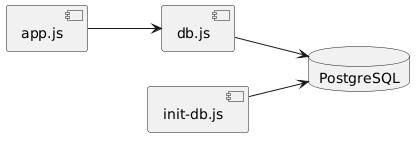
\includegraphics[width=0.8\linewidth]{images/arch-server}
	\caption{Диаграмма компонентов серверной части}
	\label{fig:arch-server}
\end{figure}

\subsubsection{Маршруты}

Маршруты API имеют общий префикс \texttt{/api}. Для административных сценариев
чтения используется query-параметр \texttt{includeHidden=1}, позволяющий получить
как опубликованные, так и скрытые записи. Основные HTTP-запросы серверной части
представлены в таблице \ref{tab:api-http}.
\begin{xltabular}{\textwidth}{|c|l|l|X|}
	\caption{Основные HTTP-запросы}
	\label{tab:api-http}
	\finishhead
	\hline
	Маршрут & Метод & Входные данные & Результат \\ \hline
	\texttt{/api/categories} & GET & --- & JSON-массив категорий \\ \hline
	\texttt{/api/categories} & POST & JSON-тело категории & Создание или обновление категории; при ошибке возвращается JSON с полем \texttt{error} \\ \hline
	\texttt{/api/places} & GET & Query-параметр & JSON-массив опубликованных мест или полный список при \texttt{includeHidden=1} \\ \hline
	\texttt{/api/places} & POST & JSON-тело места & Создание или обновление места; при ошибке возвращается JSON с полем \texttt{error} \\ \hline
	\texttt{/api/places/:id} & DELETE & \texttt{id} в URL & Удаление места; при успехе возвращается пустой ответ со статусом \texttt{204} \\ \hline
	\texttt{/api/routes} & GET & Query-параметр & JSON-массив опубликованных маршрутов с точками или полный список при \texttt{includeHidden=1} \\ \hline
	\texttt{/api/routes} & POST & JSON-тело маршрута & Создание или обновление маршрута с точками; при ошибке возвращается JSON с полем \texttt{error} \\ \hline
	\texttt{/api/routes/:id} & DELETE & \texttt{id} в URL & Удаление маршрута; при успехе возвращается пустой ответ со статусом \texttt{204} \\ \hline
\end{xltabular}

Пример успешного ответа \texttt{GET /api/categories}:
\begin{verbatim}
	[
	{
		"slug": "parks",
		"label": "Парки"
	}
	]
\end{verbatim}

Пример успешного ответа \texttt{POST /api/categories}:
\begin{verbatim}
	{
		"slug": "museums",
		"label": "Музеи"
	}
\end{verbatim}

Возможное сообщение об ошибке для \texttt{POST /api/categories}:
\begin{verbatim}
	{
		"error": "slug and label are required"
	}
\end{verbatim}

Пример успешного ответа \texttt{GET /api/places} и
\texttt{GET /api/places?includeHidden=1}:
\begin{verbatim}
	[
	{
		"id": "krasnaya-ploshchad",
		"name": "Красная площадь",
		"category": "attractions",
		"description": "Центральная площадь Курска",
		"object_info": "Исторический центр города",
		"lat": "51.730100",
		"lon": "36.193900",
		"cover_image_url": "image.com",
		"gallery": ["images/krasnaya.jpg"],
		"address": "г. Курск, Красная площадь",
		"open_hours": "Круглосуточно",
		"phone": "",
		"website_url": "",
		"visible": true,
		"updated_at": "2026-05-07T10:00:00.000Z"
	}
	]
\end{verbatim}

Пример успешного ответа \texttt{POST /api/places}:
\begin{verbatim}
	{
		"id": "krasnaya-ploshchad",
		"name": "Красная площадь",
		"category": "attractions",
		"description": "Центральная площадь Курска",
		"object_info": "Исторический центр города",
		"lat": "51.730100",
		"lon": "36.193900",
		"cover_image_url": "image.com",
		"gallery": ["images/krasnaya.jpg"],
		"address": "г. Курск, Красная площадь",
		"open_hours": "Круглосуточно",
		"phone": "",
		"website_url": "",
		"visible": true,
		"updated_at": "2026-05-07T10:00:00.000Z"
	}
\end{verbatim}

Для \texttt{DELETE /api/places/:id} при успешном выполнении сервер возвращает
статус \texttt{204 No Content}; JSON-тело ответа отсутствует.

Пример успешного ответа \texttt{GET /api/routes} и
\texttt{GET /api/routes?includeHidden=1}:
\begin{verbatim}
	[
	{
		"id": "historic-center",
		"name": "Исторический центр",
		"short_description": "Пешеходный маршрут по центру Курска",
		"description": "Маршрут объединяет ключевые городские достопримечательности.",
		"visible": true,
		"updated_at": "2026-05-07T10:00:00.000Z",
		"points": [
		{
			"place_id": "krasnaya-ploshchad",
			"position": 0,
			"place_name": "Красная площадь",
			"lat": "51.730100",
			"lon": "36.193900",
			"cover_image_url": "image.com",
			"category": "attractions"
		}
		]
	}
	]
\end{verbatim}

Пример успешного ответа \texttt{POST /api/routes}:
\begin{verbatim}
	{
		"id": "historic-center",
		"name": "Исторический центр",
		"short_description": "Пешеходный маршрут по центру Курска",
		"description": "Маршрут объединяет ключевые городские достопримечательности.",
		"visible": true,
		"updated_at": "2026-05-07T10:00:00.000Z",
		"points": [
		{
			"place_id": "krasnaya-ploshchad",
			"position": 0,
			"place_name": "Красная площадь",
			"lat": "51.730100",
			"lon": "36.193900",
			"cover_image_url": "image.com",
			"category": "attractions"
		},
		{
			"place_id": "znamsobor",
			"position": 1,
			"place_name": "Знаменский собор",
			"lat": "51.730900",
			"lon": "36.191800",
			"cover_image_url": "image.com",
			"category": "religion"
		}
		]
	}
\end{verbatim}

Возможные сообщения об ошибках для \texttt{POST /api/routes}:
\begin{verbatim}
	{
		"error": "Route name is required"
	}
\end{verbatim}

\begin{verbatim}
	{
		"error": "Route must contain at least start and end points"
	}
\end{verbatim}

Для \texttt{DELETE /api/routes/:id} при успешном выполнении сервер возвращает
статус \texttt{204 No Content}; JSON-тело ответа отсутствует.

Общий формат ошибки для обработчиков API:
\begin{verbatim}
	{
		"error": "текст ошибки"
	}
\end{verbatim}

Помимо перечисленных ошибок валидации, сервер может вернуть JSON-ответ со
статусом \texttt{500}, если произошла внутренняя ошибка приложения или ошибка
доступа к базе данных. В этом случае поле \texttt{error} содержит текст ошибки,
полученный обработчиком Express или транзакционным обработчиком сохранения
маршрута.

\subsubsection{Детализация функциональных подсистем}
Подсистема «Каталог мест» обеспечивает основной сценарий ознакомления
пользователя с содержанием платформы. Функционально она включает три слоя:
слой выдачи данных API, слой клиентской фильтрации и слой визуализации карточек.

На серверной стороне запрос \texttt{GET /api/places} возвращает только опубликованные
записи (\texttt{visible = true}), что реализует безопасность представления контента:
черновые или временно скрытые объекты не попадают в публичный интерфейс.
Административный режим использует \texttt{GET /api/places?includeHidden=1},
позволяющий работать с полным набором данных.

На клиентской стороне фильтрация по категориям реализована без повторного запроса
в БД для каждого клика, что уменьшает сетевые задержки. Такой подход рационален
для текущего объёма данных, характерного для городского гида. При дальнейшем росте
набора мест (например, на порядок) возможен переход к серверной фильтрации с
передачей параметров в API.

Подсистема маршрутов решает две взаимосвязанные задачи: хранение структуры
маршрута и визуализация последовательности точек. В техническом проекте это
реализовано через пару сущностей \texttt{routes} и \texttt{route\_points}, где
\texttt{route\_points.position} задаёт порядок прохождения.

Запрос \texttt{GET /api/routes} использует агрегацию точек в JSON-структуру.
Это уменьшает число клиентских запросов и сокращает объём «склейки» данных на
фронтенде. Компромисс такого решения --- более сложный SQL на стороне сервера,
однако выигрыш в целостности и предсказуемости ответа для UI является существенным.

Сохранение маршрута выполняется транзакционно, что особенно важно при операциях
редактирования. Если бы обновление маршрута и точек выполнялось раздельно без
транзакции, при сбое система могла бы получить маршрут без точек либо с частичным
набором точек, что нарушило бы корректность пользовательского сценария.

Административная подсистема включает операции CRUD для категорий, мест и маршрутов.
Ключевым инженерным требованием является устойчивость к невалидному вводу.
Поэтому в проекте предусмотрена двухуровневая валидация:
\begin{enumerate}
	\item Первичная --- на уровне формы и клиентской логики.
	\item Окончательная --- на уровне API перед выполнением SQL-операций.
\end{enumerate}

Серверная валидация обязательна даже при наличии клиентской, поскольку клиентский
код потенциально может быть изменён пользователем. Таким образом, архитектура
ориентирована на модель «не доверять клиенту».

\subsection{Проект базы данных программно-информационной системы}
Проект базы данных описывает логическую модель хранения категорий, объектов,
маршрутов и точек маршрутов. Схема ориентирована на реляционное хранение данных
и поддержку ссылочной целостности между основными сущностями.

\subsubsection{Компоненты базы данных}
Уровень данных построен на PostgreSQL и включает таблицы \texttt{categories},
\texttt{places}, \texttt{routes}, \texttt{route\_points}. Для маршрутов реализована связь
«один-ко-многим»: один маршрут содержит множество точек, каждая точка
ссылается на конкретный объект (place).

При сохранении маршрута операции выполняются в транзакции:
\begin{enumerate}
	\item Создаётся/обновляется запись маршрута.
	\item Удаляются старые точки маршрута.
	\item Вставляется новая последовательность точек.
\end{enumerate}
Это обеспечивает целостность данных и отсутствие «частично сохранённых» маршрутов.

Диаграмма компонентов уровня данных приведена на рисунке~\ref{fig:arch-db}.

\begin{figure}[H]
	\centering
	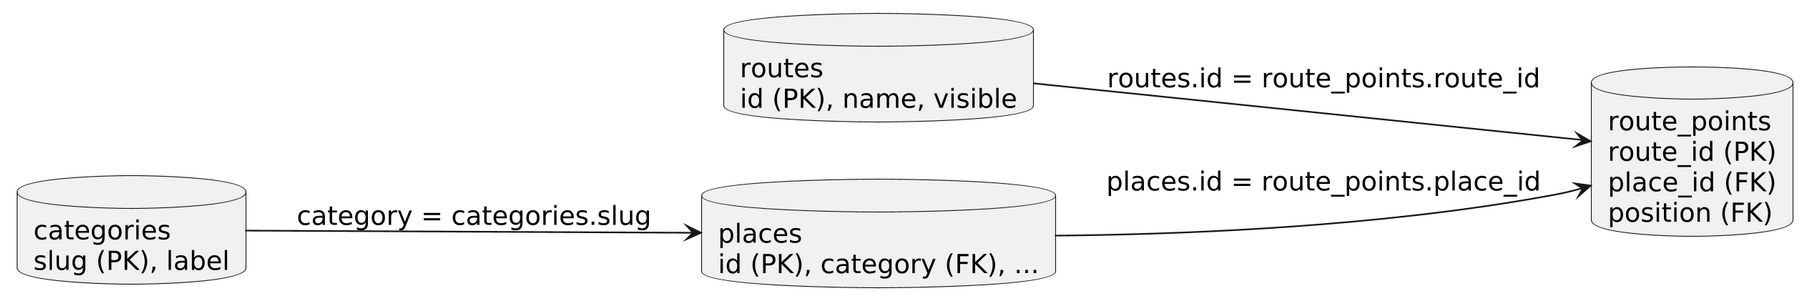
\includegraphics[width=1\linewidth, height=3.5cm]{images/arch-db}
	\caption{Диаграмма компонентов базы данных}
	\label{fig:arch-db}
\end{figure}

\subsubsection{ER-модель данных}
Ключевые сущности базы данных:
\begin{enumerate}
	\item \texttt{categories} --- справочник категорий объектов.
	\item \texttt{places} --- карточки мест (координаты, описания, контакты, видимость).
	\item \texttt{routes} --- маршруты (название, описания, видимость).
	\item \texttt{route\_points} --- точки маршрутов и их порядок.
\end{enumerate}

Связи между сущностями следующие:
\begin{enumerate}
	\item \texttt{categories (1) --- (N) places}.
	\item \texttt{routes (1) --- (N) route\_points}.
	\item \texttt{places (1) --- (N) route\_points}.
\end{enumerate}

ER-диаграмма приведена на рисунке~\ref{fig:db-er}.
\begin{figure}[H]
	\centering
	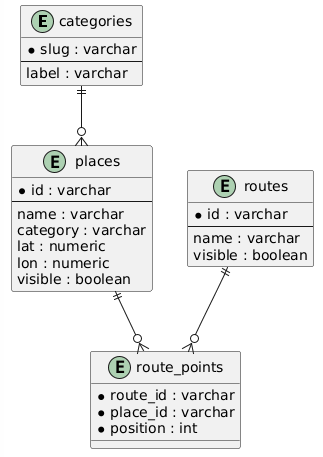
\includegraphics[width=0.45\linewidth, height=10cm]{images/db-er}
	\caption{ER-диаграмма базы данных}
	\label{fig:db-er}
\end{figure}

\subsubsection{Нормализация}
Схема данных приведена к третьей нормальной форме:
\begin{itemize}
	\item справочные значения категорий вынесены в отдельную таблицу;
	\item маршрут и его точки разделены на отдельные сущности;
	\item порядок точек хранится отдельным атрибутом \texttt{position};
	\item отсутствуют повторяющиеся группы атрибутов в одной таблице.
\end{itemize}

Нормализация снижает риск противоречивого хранения данных. Например, категория
объекта хранится в отдельной таблице, а маршрут не содержит повторяющиеся поля
мест: вместо этого используется связующая таблица \texttt{route\_points}.

\subsubsection{Реляционная модель данных}
Реляционная модель включает:
\begin{itemize}
	\item первичные ключи в каждой таблице;
	\item внешние ключи для связей между таблицами;
	\item ограничения уникальности (например, уникальный \texttt{slug} категории);
	\item флаги видимости для публикации/скрытия контента.
\end{itemize}

Для маршрутов используется составной первичный ключ \texttt{(route\_id, position)},
что обеспечивает уникальность позиции точки внутри конкретного маршрута.
Связь с таблицей \texttt{places} не допускает добавления в маршрут несуществующего
объекта.

\subsubsection{Описание структуры таблиц}
В таблицах~\ref{tab:categories}–\ref{tab:route-points} приведено описание структуры таблиц базы данных.
\begin{xltabular}{\textwidth}{|c|c|l|l|X|}
	\caption{Атрибуты таблицы «categories»}
	\label{tab:categories}
	\finishhead
	\hline
	Key Type & Optionality & Column name & Data Type & Size \\ \hline
	PK & * & slug & VARCHAR & 80 \\ \hline
	& * & label & VARCHAR & 200 \\ \hline
\end{xltabular}

\begin{xltabular}{\textwidth}{|c|c|l|l|X|}
	\caption{Атрибуты таблицы «places»}
	\label{tab:places}
	\finishhead
	\hline
	Key Type & Optionality & Column name & Data Type & Size \\ \hline
	PK & * & id & VARCHAR & 80 \\ \hline
	& * & name & VARCHAR & 255 \\ \hline
	& * & category & VARCHAR & 80 \\ \hline
	& * & description & TEXT &  \\ \hline
	&  & object\_info & TEXT & \\ \hline
	&  & lat & NUMERIC & 10,6 \\ \hline
	&  & lon & NUMERIC & 10,6 \\ \hline
	& * & cover\_image\_url & TEXT &  \\ \hline
	& * & gallery & JSONB &  \\ \hline
	&  & address & VARCHAR & 255 \\ \hline
	&  & open\_hours & VARCHAR & 120 \\ \hline
	&  & phone & VARCHAR & 12 \\ \hline
	&  & website\_url & VARCHAR & 255 \\ \hline
	& * & visible & BOOLEAN & \\ \hline
	& * & updated\_at & TIMESTAMPT & yyyy-mm-dd
	hh:mm:ss \\ \hline
\end{xltabular}

\begin{xltabular}{\textwidth}{|c|c|l|l|X|}
	\caption{Атрибуты таблицы «routes»}
	\label{tab:routes}
	\finishhead
	\hline
	Key Type & Optionality & Column name & Data Type & Size \\ \hline
	PK & * & id & VARCHAR & 80 \\ \hline
	& * & name & VARCHAR & 255 \\ \hline
	&   & short\_description & TEXT &  \\ \hline
	&   & description & TEXT &  \\ \hline
	& * & visible & BOOLEAN & \\ \hline
	& * & updated\_at & TIMESTAMPT & yyyy-mm-dd
	hh:mm:s \\ \hline
\end{xltabular}

\begin{xltabular}{\textwidth}{|c|c|l|l|X|}
	\caption{Атрибуты таблицы «route\_points»}
	\label{tab:route-points}
	\finishhead
	\hline
	Key Type & Optionality & Column name & Data Type & Size \\ \hline
	PK & * & route\_id & VARCHAR & 80 \\ \hline
	FK & * & place\_id & VARCHAR & 80 \\ \hline
	FK & * & position & INTEGER &  \\ \hline
\end{xltabular}

\subsubsection{Детализация SQL-запросов и операций доступа к данным}
Запросы чтения разделены на пользовательские и административные профили.
Пользовательский профиль ограничивает выдачу опубликованным контентом, тогда как
административный позволяет видеть все записи. Такое разграничение реализуется
без дублирования таблиц и без усложнения схемы БД.

Для маршрутов применяется \texttt{LEFT JOIN} с таблицей точек и таблицей мест,
что позволяет формировать полный ответ даже в случае частичной неполноты связанных
данных. Дополнительно используется сортировка по \texttt{updated\_at DESC},
обеспечивающая приоритет актуального контента в выдаче.

Операции записи для мест и маршрутов реализованы в стиле \texttt{UPSERT}
(\texttt{INSERT ... ON CONFLICT DO UPDATE}). Это снижает вероятность ошибок при
повторных сохранениях и упрощает клиентскую логику: интерфейсу не требуется
разделять технические ветки «создать» и «обновить» на уровне разных endpoint'ов.

Удаление выполняется через \texttt{DELETE} по идентификатору сущности.
Для маршрутов удаление основной записи приводит к удалению связанных точек
маршрута согласно ограничениям целостности (при настроенном каскаде) либо через
явное удаление в транзакционном блоке.

Основные риски SQL-слоя:
\begin{itemize}
	\item SQL-инъекции при небезопасной конкатенации строк;
	\item «потерянные обновления» при конкурентном редактировании;
	\item рост времени ответа при увеличении объёма данных.
\end{itemize}

В проекте применяются параметризованные запросы, что устраняет риск SQL-инъекций.
Для минимизации конкурентных рисков критичные операции объединяются в транзакции.
При росте нагрузки проектом предусмотрен путь эволюции: индексация полей поиска,
аудит планов запросов и вынос тяжёлых отчётных выборок в отдельные представления.

\subsection{Надёжность, производительность и масштабирование}

\subsubsection{Надёжность транзакционных операций}
Сценарий сохранения маршрута реализован в явной транзакции PostgreSQL
(\texttt{BEGIN/COMMIT/ROLLBACK}), что гарантирует атомарность изменения маршрута
и его точек. При ошибке любой операции состояние БД откатывается.

\subsubsection{Оптимизация запросов чтения}
Для получения маршрутов применяется SQL-агрегация в JSON, что уменьшает
количество round-trip между сервером и клиентом и снижает необходимость
дополнительных клиентских запросов для каждой точки маршрута.

\subsubsection{Потенциал горизонтального масштабирования}
Текущая архитектура допускает дальнейшее масштабирование:
\begin{itemize}
	\item вынос PostgreSQL на отдельный сервер;
	\item запуск нескольких экземпляров Node.js;
	\item добавление кэширования для часто запрашиваемых read-only данных
	(справочники категорий и опубликованные карточки).
\end{itemize}

\subsection{Информационная безопасность технического проекта}

\subsubsection{Профиль угроз}
Для проекта релевантны угрозы:
\begin{itemize}
	\item несанкционированное изменение контента через админ-страницу;
	\item отправка некорректных/вредоносных данных в API;
	\item раскрытие внутренних ошибок сервера.
\end{itemize}

\subsubsection{Меры защиты}
В техническом проекте применяются следующие меры:
\begin{itemize}
	\item параметризованные SQL-запросы в серверном слое;
	\item валидация обязательных полей и ограничений бизнес-логики;
	\item централизованная обработка ошибок без утечки стек-трейсов в клиент;
	\item ограничение доступа к \texttt{pages/admin.html} на уровне инфраструктуры
	(allowlist, базовая аутентификация).
\end{itemize}

\subsection{Эксплуатация и развёртывание}

\subsubsection{Локальное развёртывание}
Базовый сценарий развёртывания:
\begin{enumerate}
	\item Установить зависимости \texttt{npm install}.
	\item Настроить \texttt{DATABASE\_URL}.
	\item Выполнить инициализацию схемы \texttt{npm run db:init}.
	\item Запустить сервер \texttt{npm run start}.
	\item Открыть пользовательские и административные страницы в браузере.
\end{enumerate}

\subsubsection{Параметры конфигурации}
Ключевые параметры окружения:
\begin{enumerate}
	\item \texttt{DATABASE\_URL} --- строка подключения к PostgreSQL.
	\item \texttt{PORT} --- порт HTTP-сервера (по умолчанию 3000).
	\item \texttt{window.API\_BASE\_URL} во фронтенде --- адрес backend API
	при разделении фронта и бэкенда по доменам.
\end{enumerate}

\subsubsection{Конфигурация технических средств}
Для развёртывания и эксплуатации системы требуется:
\begin{enumerate}
	\item Сервер/ПК с установленными Node.js и PostgreSQL;
	\item Доступ к сети для загрузки картографического API;
	\item Современный веб-браузер для пользователей и администратора.
\end{enumerate}

Рекомендуемая минимальная конфигурация:
\begin{enumerate}
	\item Процессор: от 2 ГГц;
	\item ОЗУ: от 4 ГБ;
	\item Свободное место на диске: от 500 МБ (без учёта роста БД).
\end{enumerate}

\subsubsection{Наблюдаемость и сопровождение}
Для поддержки эксплуатационного цикла рекомендуется:
\begin{itemize}
	\item централизованный сбор логов Node.js;
	\item регулярные бэкапы PostgreSQL;
	\item smoke-проверки API после деплоя;
	\item периодический аудит контента и ссылок (валидность URL и изображений).
\end{itemize}

\subsection{Верификация технического проекта}

\subsubsection{Функциональная верификация}
Функциональная верификация должна покрывать:
\begin{itemize}
	\item пользовательские сценарии просмотра и фильтрации;
	\item административные сценарии CRUD для мест и маршрутов;
	\item корректность включения/исключения скрытого контента;
	\item устойчивость к невалидным входным данным.
\end{itemize}

\subsubsection{Техническая верификация}
Техническая верификация должна включать:
\begin{itemize}
	\item проверку целостности БД после транзакционных операций;
	\item проверку корректности HTTP-кодов и формата ошибок;
	\item проверку работы карты и модальных окон в поддерживаемых браузерах;
	\item проверку производительности при росте объёма контента.
\end{itemize}
